% Provenance (never printed): cycle 3 "La planete Terre. Les etres vivants
% dans leur environnement" (natural phenomena: volcanoes and earthquakes,
% natural hazards and the behaviour to adopt); see sources/book1/PROVENANCE.md.
% Book 1, grade 4, chapter 2.
\chapter{Volcanes y terremotos: una primera mirada}\label{ch:g4:volcanoes-earthquakes-first-look}

El lunes por la noche, las noticias muestran un \omterm{def:g4:volcanoes-earthquakes-first-look:volcano}{volcán} en una isla lejana.
En la oscuridad, un surtidor de \omterm{def:g3:stones-pebbles-sand:rock}{roca} incandescente de color naranja brota de
una grieta del suelo, y unos \omterm{def:g1:landscapes-around-us:water}{ríos} de fuego bajan despacio por la ladera
hasta el \omterm{def:g2:water-on-earth:ocean}{mar}, silbando y echando vapor. El jueves, las noticias muestran
otro lugar: un pueblo donde, al amanecer, el suelo tembló durante medio
minuto. Las chimeneas cayeron a la calle y una casa vieja se salió de sus
cimientos.

Son dos sucesos muy distintos. Y sin embargo los dos vienen del interior
profundo de la Tierra y, como veremos, los dos ocurren mucho más a menudo
en unas partes del mundo que en otras.

\begin{recall}
Las \omterm{def:g1:landscapes-around-us:landform}{montañas}, las \omterm{def:g1:landscapes-around-us:landform}{colinas}, los \omterm{def:g1:landscapes-around-us:landform}{valles} y las \omterm{def:g1:landscapes-around-us:landform}{llanuras} son las formas del
terreno (\cref{ch:g1:landscapes-around-us}). La tierra firme está reunida en
siete \omterm{def:g3:continents-and-oceans:continent}{continentes}, entre cinco \omterm{def:g2:water-on-earth:ocean}{océanos}; el Pacífico es el \omterm{def:g2:water-on-earth:ocean}{océano} más grande
(\cref{ch:g3:continents-and-oceans}).
\end{recall}

\section{Un volcán entra en erupción}

Muy por debajo de nuestros pies, la Tierra está muy caliente. En algunos
lugares, la \omterm{def:g3:stones-pebbles-sand:rock}{roca} de allí abajo está tan caliente que se ha fundido. Esta
\omterm{def:g3:stones-pebbles-sand:rock}{roca} fundida es más ligera que la \omterm{def:g3:stones-pebbles-sand:rock}{roca} sólida que la rodea, así que sube
despacio, como un corcho en el agua. Donde encuentra una salida a la
superficie, nace un \omterm{def:g4:volcanoes-earthquakes-first-look:volcano}{volcán}.

\begin{definition}[Volcán]\label{def:g4:volcanoes-earthquakes-first-look:volcano}
Un \emph{volcán}\index{volcan@volcán} es un lugar por donde sale a la
superficie \omterm{def:g3:stones-pebbles-sand:rock}{roca} fundida del interior profundo de la Tierra, y también la
\omterm{def:g1:landscapes-around-us:landform}{colina} o la \omterm{def:g1:landscapes-around-us:landform}{montaña} que esa \omterm{def:g3:stones-pebbles-sand:rock}{roca} fundida construye allí, capa tras capa.
\end{definition}

\begin{definition}[Erupción, lava y ceniza volcánica]\label{def:g4:volcanoes-earthquakes-first-look:eruption}
Una \emph{erupción}\index{erupcion@erupción} es el momento en que un \omterm{def:g4:volcanoes-earthquakes-first-look:volcano}{volcán}
expulsa \omterm{def:g3:stones-pebbles-sand:rock}{roca} fundida, ceniza y gas. La \emph{lava}\index{lava} es la \omterm{def:g3:stones-pebbles-sand:rock}{roca}
fundida que se derrama por la superficie; corre, y luego se enfría y se
endurece hasta convertirse en \omterm{def:g3:stones-pebbles-sand:rock}{roca} nueva. La \emph{ceniza
volcánica}\index{ceniza volcanica@ceniza volcánica} está hecha de trocitos
diminutos de \omterm{def:g3:stones-pebbles-sand:rock}{roca} y de vidrio lanzados al aire por una erupción; vuelve a
caer como una \omterm{def:g4:clouds-rain-snow:precipitation}{nieve} gris.
\end{definition}

\begin{omfigure}
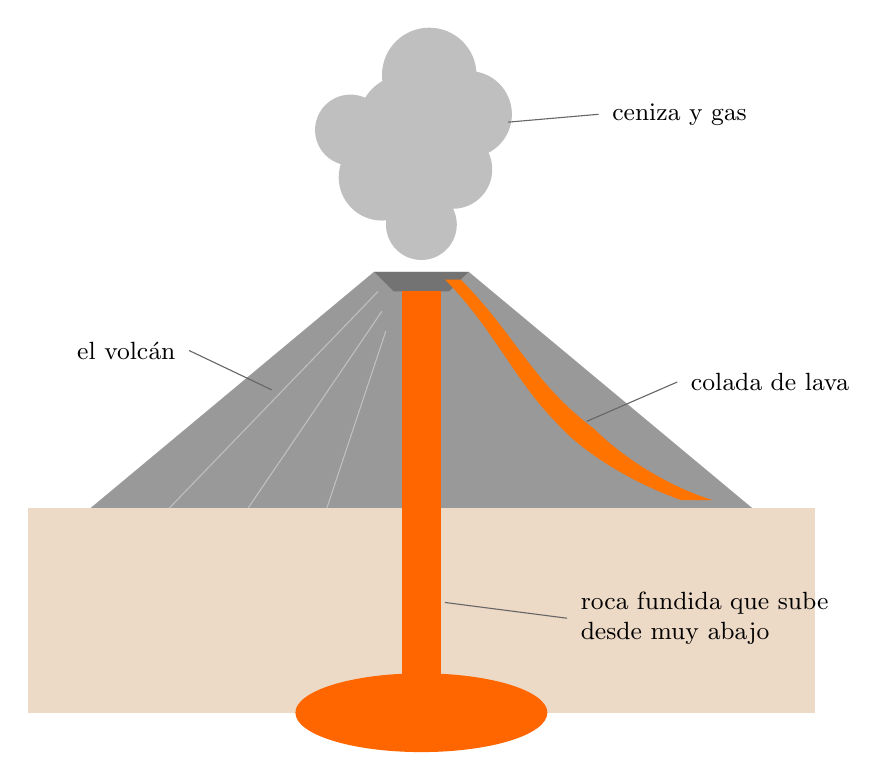
\begin{tikzpicture}[font=\small]
  % ground and deep rock
  \fill[brown!30] (-5,-2.6) rectangle (5,0);
  % the volcano
  \fill[black!40] (-4.2,0) -- (-0.6,3.0) -- (0.6,3.0) -- (4.2,0) -- cycle;
  \fill[black!55] (-0.6,3.0) -- (-0.35,2.75) -- (0.35,2.75) -- (0.6,3.0) -- cycle;
  % layers inside the cone
  \foreach \k in {1,2,3}
    \draw[black!25] (-4.2+1.0*\k,0) -- (-0.6+0.05*\k,3.0-0.25*\k);
  % molten rock rising from deep below
  \fill[orange!80!red] (-0.25,-2.6) -- (-0.25,2.75) -- (0.25,2.75) -- (0.25,-2.6) -- cycle;
  \fill[orange!80!red] (0,-2.6) ellipse (1.6 and 0.5);
  % lava flow on the right flank
  \fill[orange!90!red] (0.5,2.9) .. controls (1.2,2.2) and (1.4,1.6) .. (2.2,1.0)
    .. controls (2.6,0.6) and (3.2,0.25) .. (3.7,0.1) -- (3.3,0.1)
    .. controls (2.6,0.35) and (2.0,0.75) .. (1.7,1.1)
    .. controls (1.2,1.6) and (0.9,2.3) .. (0.3,2.9) -- cycle;
  % ash and gas cloud
  \foreach \x/\y/\r in {0/3.6/0.45, -0.5/4.2/0.55, 0.4/4.3/0.5, -0.2/4.9/0.6, 0.6/5.0/0.55, -0.9/4.8/0.45, 0.1/5.5/0.6}
    \fill[black!25] (\x,\y) circle (\r);
  % labels
  \node[anchor=west] at (2.3,5.0) {ceniza y gas};
  \draw[black!60] (2.25,5.0) -- (1.1,4.9);
  \node[anchor=west] at (3.3,1.6) {colada de lava};
  \draw[black!60] (3.25,1.6) -- (2.1,1.1);
  \node[anchor=east] at (-3.0,2.0) {el volcán};
  \draw[black!60] (-2.95,2.0) -- (-1.9,1.5);
  \node[anchor=west, align=left] at (1.9,-1.4) {roca fundida que sube\\desde muy abajo};
  \draw[black!60] (1.85,-1.4) -- (0.3,-1.2);
\end{tikzpicture}

{\small Un \omterm{def:g4:volcanoes-earthquakes-first-look:volcano}{volcán} en \omterm{def:g4:volcanoes-earthquakes-first-look:eruption}{erupción} (dibujo, sin escala). La \omterm{def:g3:stones-pebbles-sand:rock}{roca} fundida sube
desde muy abajo y sale por arriba: baja como \omterm{def:g4:volcanoes-earthquakes-first-look:eruption}{lava}, mientras que la ceniza y
el gas salen disparados hacia el cielo. Cada \omterm{def:g4:volcanoes-earthquakes-first-look:eruption}{erupción} añade una capa nueva
a la \omterm{def:g1:landscapes-around-us:landform}{montaña}.}
\label{fig:g4:volcanoes-earthquakes-first-look:volcano}
\end{omfigure}

No todas las \omterm{def:g4:volcanoes-earthquakes-first-look:eruption}{erupciones} son iguales. En algunas, la \omterm{def:g4:volcanoes-earthquakes-first-look:eruption}{lava} es fluida: sale
tranquilamente en \omterm{def:g1:landscapes-around-us:water}{ríos} incandescentes que pueden recorrer kilómetros, a
veces hasta el \omterm{def:g2:water-on-earth:ocean}{mar}. En otras, la \omterm{def:g3:stones-pebbles-sand:rock}{roca} fundida es espesa y está llena de
gas, como una botella de refresco agitada: cuando sale, estalla en una
enorme columna de ceniza que sube muy alto en el cielo.

\begin{omfigure}
\begin{minipage}[b]{0.56\linewidth}\centering
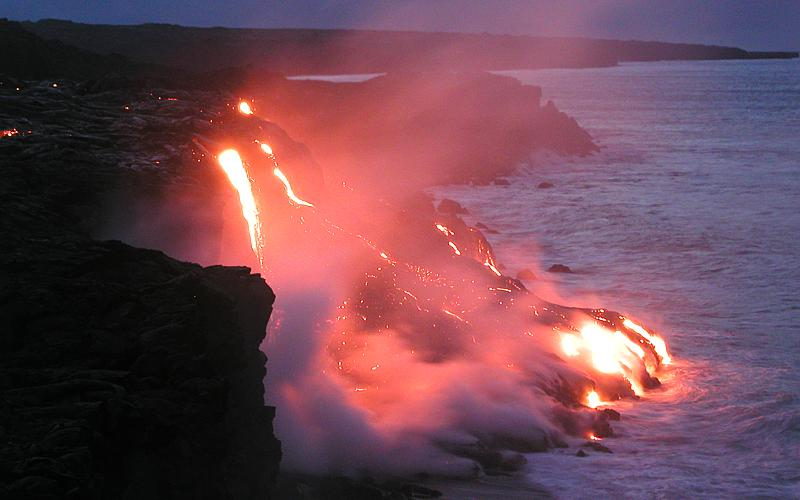
\includegraphics[width=\linewidth]{images/book1/g4-lava-ocean.jpg}

{\small Una \omterm{def:g4:volcanoes-earthquakes-first-look:eruption}{erupción} tranquila: la \omterm{def:g4:volcanoes-earthquakes-first-look:eruption}{lava} cae por un acantilado al \omterm{def:g2:water-on-earth:ocean}{océano}, en
Hawái. Fotografía: Observatorio Volcánico de Hawái del USGS (dominio
público).}
\end{minipage}\hfill
\begin{minipage}[b]{0.4\linewidth}\centering
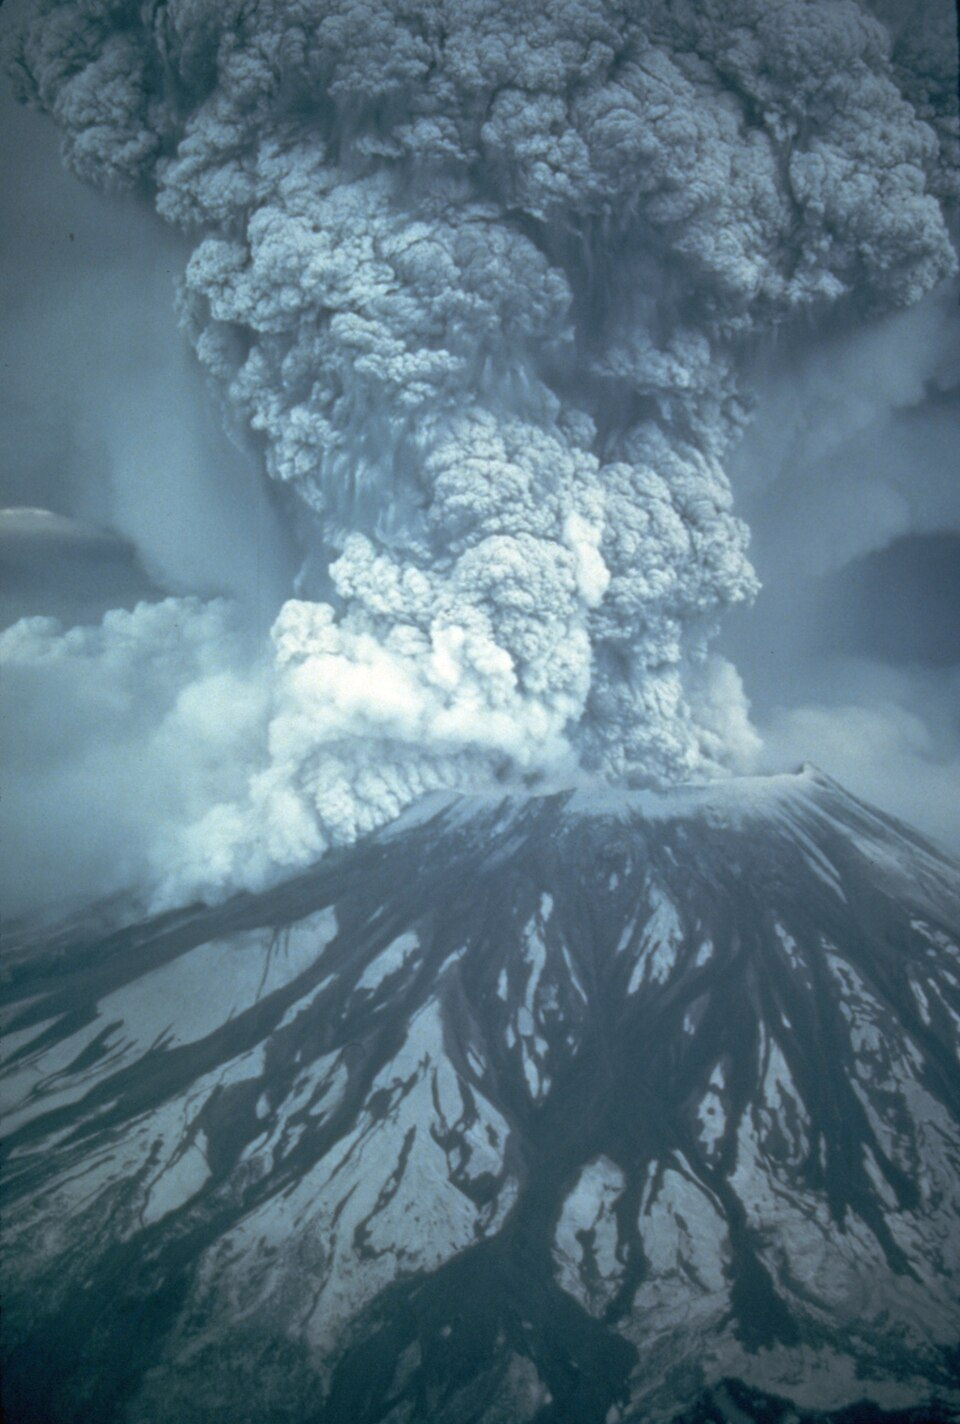
\includegraphics[width=0.78\linewidth]{images/book1/g4-st-helens.jpg}

{\small Una \omterm{def:g4:volcanoes-earthquakes-first-look:eruption}{erupción} explosiva: el monte Santa Helena, Estados Unidos, 18~de
mayo de 1980. Fotografía: Austin Post, USGS (dominio público).}
\end{minipage}
% ledger: usgs:pu-oo-ocean, usgs:msh-1980
\label{fig:g4:volcanoes-earthquakes-first-look:two-eruptions}
\end{omfigure}

\begin{example}[El monte Santa Helena, 1980]\label{ex:g4:volcanoes-earthquakes-first-look:st-helens}
En la primavera de 1980 se formó un abultamiento en la ladera del monte
Santa Helena, porque la \omterm{def:g3:stones-pebbles-sand:rock}{roca} fundida empujaba hacia arriba dentro de la
\omterm{def:g1:landscapes-around-us:landform}{montaña}. La mañana del 18~de mayo, un pequeño \omterm{def:g4:volcanoes-earthquakes-first-look:earthquake}{terremoto} sacudió la \omterm{def:g1:landscapes-around-us:landform}{montaña},
el abultamiento se desprendió en un deslizamiento gigantesco y el \omterm{def:g4:volcanoes-earthquakes-first-look:volcano}{volcán}
estalló hacia un lado y hacia arriba. Los 400~metros de arriba de la
\omterm{def:g1:landscapes-around-us:landform}{montaña} desaparecieron: la cima se convirtió en un cráter enorme.
% ledger: usgs:msh-1980
\end{example}

\section{El suelo tiembla}

Las \omterm{def:g3:stones-pebbles-sand:rock}{rocas} de muy por debajo de nuestros pies no están del todo quietas. Muy
despacio, las empujan y tiran de ellas. Se doblan un poco, como una regla
que empujas por los dos extremos --- hasta que, de repente, se rompen y se
deslizan. La sacudida hace temblar el suelo kilómetros a la redonda.

\begin{definition}[Terremoto]\label{def:g4:volcanoes-earthquakes-first-look:earthquake}
Un \emph{terremoto}\index{terremoto} es una sacudida repentina del suelo,
causada por \omterm{def:g3:stones-pebbles-sand:rock}{rocas} que se rompen y se deslizan en las profundidades.
\end{definition}

Un \omterm{def:g4:volcanoes-earthquakes-first-look:earthquake}{terremoto} suele durar solo unos segundos, a veces un minuto o dos en los
más grandes. La mayoría de los \omterm{def:g4:volcanoes-earthquakes-first-look:earthquake}{terremotos} son tan pequeños que nadie los
nota: solo los detectan los instrumentos. Uno fuerte puede hacer que el
suelo se balancee como la cubierta de un barco, agrietar las carreteras y
derribar muros y casas.

\begin{omfigure}
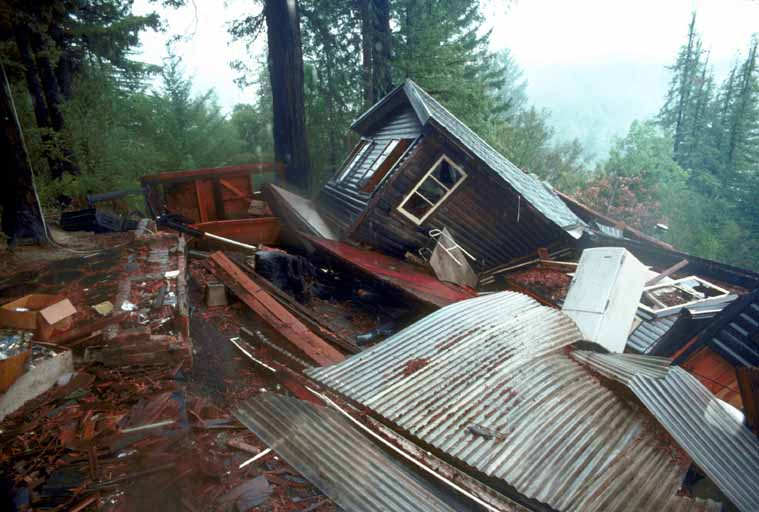
\includegraphics[width=0.55\linewidth]{images/book1/g4-loma-prieta-house.jpg}

{\small Tras un fuerte \omterm{def:g4:volcanoes-earthquakes-first-look:earthquake}{terremoto} en California en 1989: esta casa de
madera salió despedida de lado y cayó de su base de hormigón. Fotografía:
J.~K.~Nakata, USGS (dominio público).}
% ledger: usgs:loma-prieta-house
\end{omfigure}

\begin{remark}[¿Con qué frecuencia?]\label{rem:g4:volcanoes-earthquakes-first-look:how-often}
Los geólogos llevan una lista de todos los grandes \omterm{def:g4:volcanoes-earthquakes-first-look:earthquake}{terremotos} de la Tierra.
En los 50 años que van de 1976 a 2025, la lista cuenta 7\,031 grandes
\omterm{def:g4:volcanoes-earthquakes-first-look:earthquake}{terremotos} (lo bastante fuertes para dañar los edificios cercanos): unos
141 al año, o casi 3 cada semana. Los más grandes de todos, que pueden
destruir ciudades enteras, son unos 14 al año. En esa misma Tierra, unos
1\,200 \omterm{def:g4:volcanoes-earthquakes-first-look:volcano}{volcanes} han entrado en \omterm{def:g4:volcanoes-earthquakes-first-look:eruption}{erupción} en los últimos doce mil años, más o
menos.
% ledger: data:usgs-comcat, data:gvp
\end{remark}

\section{Dónde hay volcanes y terremotos}

Si los \omterm{def:g4:volcanoes-earthquakes-first-look:volcano}{volcanes} y los \omterm{def:g4:volcanoes-earthquakes-first-look:earthquake}{terremotos} ocurrieran en cualquier sitio al azar, los
puntos de un \omterm{def:g3:continents-and-oceans:world-map}{mapamundi} estarían repartidos por igual. No lo están.

El \omterm{def:g2:drawing-to-map:map}{mapa} de abajo muestra una disposición llamativa. Casi todos los \omterm{def:g4:volcanoes-earthquakes-first-look:volcano}{volcanes}
y casi todos los grandes \omterm{def:g4:volcanoes-earthquakes-first-look:earthquake}{terremotos} están en franjas largas y estrechas.
La más larga de todas rodea el \omterm{def:g2:water-on-earth:ocean}{océano} Pacífico: desde Nueva Zelanda sube
por Indonesia, Filipinas y Japón, cruza hasta Alaska y baja luego por toda
la \omterm{def:g1:landscapes-around-us:water}{costa} oeste de América hasta la punta de Chile. Por sus muchos \omterm{def:g4:volcanoes-earthquakes-first-look:volcano}{volcanes},
se la suele llamar el ``Anillo de Fuego''.

\begin{example}[Contamos en el mapa]\label{ex:g4:volcanoes-earthquakes-first-look:shares}
Hemos contado los puntos que están en el anillo sombreado (a menos de
500~kilómetros de su línea central). De los 1\,214 \omterm{def:g4:volcanoes-earthquakes-first-look:volcano}{volcanes}, 837 están en el
anillo: unos 2 de cada 3. De los 696 \omterm{def:g4:volcanoes-earthquakes-first-look:earthquake}{terremotos} más grandes, 532 están en el
anillo: unos 3 de cada 4. El anillo ocupa solo una pequeña parte de la
Tierra, pero contiene la mayoría de sus \omterm{def:g4:volcanoes-earthquakes-first-look:volcano}{volcanes} y de sus \omterm{def:g4:volcanoes-earthquakes-first-look:earthquake}{terremotos}.
% ledger: data:gvp, data:usgs-comcat
\end{example}

\begin{omfigure}
\begin{tikzpicture}
\begin{axis}[ommap, width=\linewidth, xtick=\empty, ytick=\empty, grid=none,
    legend style={font=\scriptsize, at={(0.5,-0.02)}, anchor=north,
      draw=none, legend columns=3, /tikz/every even column/.append style={column sep=6pt}},
    legend cell align=left]
  \addplot[fill=omHypsLandA!85!black, draw=black!45, line width=0.2pt, forget plot]
    table {figdata/out/shared-geo-land.dat};
  \addplot[orange!80!black, opacity=0.35, line width=9pt, line cap=round, line join=round]
    table {figdata/out/grade-4-ring_of_fire-ring.dat};
  \addlegendentry{el anillo alrededor del Pacífico}
  \addplot[only marks, mark=triangle*, mark size=1.3pt, red!75!black]
    table[x=lon, y=lat] {figdata/out/grade-4-ring_of_fire-volcanoes.dat};
  \addlegendentry{un volcán (últimos 12\,000 años)}
  \addplot[only marks, mark=*, mark size=1.0pt, black, fill opacity=0.6]
    table[x=lon, y=lat] {figdata/out/grade-4-ring_of_fire-quakes7.dat};
  \addlegendentry{un terremoto muy grande (1976--2025)}
\end{axis}
\end{tikzpicture}

{\small Los \omterm{def:g4:volcanoes-earthquakes-first-look:volcano}{volcanes} que han entrado en \omterm{def:g4:volcanoes-earthquakes-first-look:eruption}{erupción} en los últimos doce mil
años, más o menos, y los \omterm{def:g4:volcanoes-earthquakes-first-look:earthquake}{terremotos} más grandes de 1976--2025. Casi todos
están a lo largo de un anillo de cadenas de islas y cordilleras alrededor
del \omterm{def:g2:water-on-earth:ocean}{océano} Pacífico (sombreado). Datos: Global Volcanism Program de la
Smithsonian; catálogo de \omterm{def:g4:volcanoes-earthquakes-first-look:earthquake}{terremotos} del Servicio Geológico de Estados
Unidos (USGS); \omterm{def:g1:landscapes-around-us:water}{costas}, Natural Earth.}
\label{fig:g4:volcanoes-earthquakes-first-look:map}
% ledger: data:gvp, data:usgs-comcat, data:ne-land
\end{omfigure}

Otras franjas son más pequeñas: una cruza el sur de Europa y de Asia, del
\omterm{def:g2:water-on-earth:ocean}{mar} Mediterráneo al Himalaya; otras recorren el centro de los \omterm{def:g2:water-on-earth:ocean}{océanos},
donde los \omterm{def:g4:volcanoes-earthquakes-first-look:volcano}{volcanes} están escondidos bajo el agua. Algunos lugares, como
Hawái, tienen \omterm{def:g4:volcanoes-earthquakes-first-look:volcano}{volcanes} lejos de cualquier franja. Por qué las franjas están
donde están es una pregunta para el \cref{ch:g7:plate-tectonics}: la
respuesta explica la forma de todo el \omterm{def:g2:drawing-to-map:map}{mapa}.

\section{Ponerse a salvo}

Nadie puede detener una \omterm{def:g4:volcanoes-earthquakes-first-look:eruption}{erupción} ni un \omterm{def:g4:volcanoes-earthquakes-first-look:earthquake}{terremoto}. Pero saber qué hacer
salva vidas.

\begin{omfigure}
\begin{tikzpicture}[font=\small, line cap=round, line join=round]
  % --- panel 1: DROP onto hands and knees
  \begin{scope}
    \draw[black!30] (-0.2,0) -- (2.8,0);
    \fill[omDef] (0.62,0.98) circle (0.21);
    \draw[omDef, line width=2.2pt] (0.88,0.98) -- (2.0,0.95);
    \draw[omDef, line width=2pt] (0.95,0.96) -- (0.95,0.05);
    \draw[omDef, line width=2pt] (2.0,0.95) -- (1.98,0.08) -- (2.65,0.08);
    \node[font=\bfseries] at (1.3,-0.45) {AGÁCHATE};
    \node[font=\scriptsize, align=center] at (1.3,-0.95) {apoyando las manos\\y las rodillas};
  \end{scope}
  % --- panel 2: COVER under a table
  \begin{scope}[xshift=4cm]
    \draw[black!30] (-0.2,0) -- (2.8,0);
    \fill[brown!60!black] (-0.1,1.45) rectangle (2.7,1.6);
    \draw[brown!60!black, line width=2pt] (0.1,1.45) -- (0.1,0) (2.5,1.45) -- (2.5,0);
    \fill[omDef] (0.75,0.95) circle (0.2);
    \draw[omDef, line width=2.2pt] (0.95,0.85) -- (1.95,0.8);
    \draw[omDef, line width=2pt] (1.9,0.8) -- (1.65,0.05) -- (2.25,0.05);
    \draw[omDef, line width=2pt] (1.0,0.85) -- (0.7,1.2) -- (0.5,0.95);
    \node[font=\bfseries] at (1.3,-0.45) {CÚBRETE};
    \node[font=\scriptsize, align=center] at (1.3,-0.95) {la cabeza y el cuello,\\bajo una mesa sólida};
  \end{scope}
  % --- panel 3: HOLD ON to the table leg
  \begin{scope}[xshift=8cm]
    \draw[black!30] (-0.2,0) -- (2.8,0);
    \fill[brown!60!black] (-0.1,1.45) rectangle (2.7,1.6);
    \draw[brown!60!black, line width=2pt] (0.1,1.45) -- (0.1,0) (2.5,1.45) -- (2.5,0);
    \fill[omDef] (0.75,0.95) circle (0.2);
    \draw[omDef, line width=2.2pt] (0.95,0.85) -- (1.95,0.8);
    \draw[omDef, line width=2pt] (1.9,0.8) -- (1.65,0.05) -- (2.25,0.05);
    \draw[omDef, line width=2pt] (1.0,0.85) -- (0.7,1.2) -- (0.5,0.95);
    \draw[omDef, line width=2pt] (1.0,0.8) -- (0.45,0.6) -- (0.12,0.65);
    \node[font=\bfseries] at (1.3,-0.45) {AGÁRRATE};
    \node[font=\scriptsize, align=center] at (1.3,-0.95) {a la mesa hasta que\\deje de temblar};
  \end{scope}
\end{tikzpicture}

{\small Lo que hay que hacer en cuanto el suelo empieza a temblar: agáchate,
cúbrete y agárrate.}
\label{fig:g4:volcanoes-earthquakes-first-look:drop-cover}
% ledger: shakeout:dch
\end{omfigure}

\begin{safety}
\textbf{En un \omterm{def:g4:volcanoes-earthquakes-first-look:earthquake}{terremoto}.} En cuanto notes que el suelo tiembla:
\textbf{agáchate} apoyando las manos y las rodillas; \textbf{cúbrete} la
cabeza y el cuello con el brazo, y métete a gatas debajo de una mesa o un
pupitre sólido si hay uno cerca; \textbf{agárrate} a él hasta que deje de
temblar. No salgas corriendo mientras el suelo tiembla, y no te quedes bajo
el marco de una puerta: los cristales y los objetos que caen son el
peligro principal. Cuando pare, sal del edificio con calma, como practicas
en los simulacros del colegio.

\textbf{Cerca de un \omterm{def:g4:volcanoes-earthquakes-first-look:volcano}{volcán}.} Los científicos vigilan los \omterm{def:g4:volcanoes-earthquakes-first-look:volcano}{volcanes} que
pueden despertar. Si avisan de que se acerca una \omterm{def:g4:volcanoes-earthquakes-first-look:eruption}{erupción}, las autoridades
piden a la gente que abandone la zona. Sigue sus instrucciones enseguida, y
no te acerques nunca para mirar.
\end{safety}
% ledger: shakeout:dch

\begin{omfigure}

\includegraphics[width=0.55\linewidth]{images/book1/ai/g4-earthquake-drill.jpg}

{\small Un simulacro de \omterm{def:g4:volcanoes-earthquakes-first-look:earthquake}{terremoto}: los alumnos practican ``agáchate,
cúbrete y agárrate'' debajo de sus mesas.}
\end{omfigure}

\section{Ejercicios}

\begin{exercise}[$\star$]\label{exo:g4:volcanoes-earthquakes-first-look:1}
¿\omterm{def:g4:volcanoes-earthquakes-first-look:eruption}{Lava}, ceniza o gas? (a) un \omterm{def:g1:landscapes-around-us:water}{río} de \omterm{def:g3:stones-pebbles-sand:rock}{roca} fundida incandescente que baja por
una ladera; (b) trocitos diminutos de \omterm{def:g3:stones-pebbles-sand:rock}{roca} lanzados al cielo, que vuelven a
caer como una \omterm{def:g4:clouds-rain-snow:precipitation}{nieve} gris; (c) algo invisible que sale del \omterm{def:g4:volcanoes-earthquakes-first-look:volcano}{volcán} con la
ceniza.
\end{exercise}

\begin{exercise}[$\star$]\label{exo:g4:volcanoes-earthquakes-first-look:2}
¿Qué es un \omterm{def:g4:volcanoes-earthquakes-first-look:earthquake}{terremoto}? ¿Dura horas o segundos?
\end{exercise}

\begin{exercise}[$\star$]\label{exo:g4:volcanoes-earthquakes-first-look:3}
Ordena los tres pasos: agárrate; agáchate; cúbrete.
\end{exercise}

\begin{exercise}[$\star$]\label{exo:g4:volcanoes-earthquakes-first-look:4}
En el \omterm{def:g2:drawing-to-map:map}{mapa} de la página~\pageref{fig:g4:volcanoes-earthquakes-first-look:map},
¿alrededor de qué \omterm{def:g2:water-on-earth:ocean}{océano} están la mayoría de los \omterm{def:g4:volcanoes-earthquakes-first-look:volcano}{volcanes}?
\end{exercise}

\begin{exercise}[$\star$]\label{exo:g4:volcanoes-earthquakes-first-look:5}
¿Verdadero o falso? (a) La mayoría de los \omterm{def:g4:volcanoes-earthquakes-first-look:earthquake}{terremotos} son demasiado pequeños
para notarlos. (b) La \omterm{def:g4:volcanoes-earthquakes-first-look:eruption}{lava} sigue líquida para siempre. (c) Cuando el suelo
tiembla, lo más seguro es salir corriendo a la calle.
\end{exercise}

\begin{exercise}[$\star$]\label{exo:g4:volcanoes-earthquakes-first-look:6}
Mira el dibujo del \omterm{def:g4:volcanoes-earthquakes-first-look:volcano}{volcán} de la página~\pageref{fig:g4:volcanoes-earthquakes-first-look:volcano}.
¿De dónde viene la \omterm{def:g3:stones-pebbles-sand:rock}{roca} fundida? ¿Por dónde sale?
\end{exercise}

\begin{exercise}[$\star\star$]\label{exo:g4:volcanoes-earthquakes-first-look:7}
En el \omterm{def:g2:drawing-to-map:map}{mapa}, busca: (a) un país de América con muchos \omterm{def:g4:volcanoes-earthquakes-first-look:volcano}{volcanes} a lo largo de
todo su territorio; (b) un grupo de islas en medio del \omterm{def:g2:water-on-earth:ocean}{océano} Pacífico, con
\omterm{def:g4:volcanoes-earthquakes-first-look:volcano}{volcanes}, que no está en el anillo.
\end{exercise}

\begin{exercise}[$\star\star$]\label{exo:g4:volcanoes-earthquakes-first-look:8}
Cada año se producen unos 141 grandes \omterm{def:g4:volcanoes-earthquakes-first-look:earthquake}{terremotos}. ¿Cuántos son, más o
menos, en un mes? (Un año tiene 12 meses; da un número entero.)
\end{exercise}

\begin{exercise}[$\star\star$]\label{exo:g4:volcanoes-earthquakes-first-look:9}
Unos 3 de cada 4 \omterm{def:g4:volcanoes-earthquakes-first-look:earthquake}{terremotos} muy grandes ocurren en el anillo alrededor del
Pacífico. De 20 \omterm{def:g4:volcanoes-earthquakes-first-look:earthquake}{terremotos} muy grandes, ¿cuántos esperarías, más o menos,
en el anillo? ¿Y fuera de él?
\end{exercise}

\begin{exercise}[$\star\star$]\label{exo:g4:volcanoes-earthquakes-first-look:10}
Durante un simulacro de \omterm{def:g4:volcanoes-earthquakes-first-look:earthquake}{terremoto}, Leo corre a ponerse bajo el marco de la
puerta del aula. ¿Qué debería haber hecho, y por qué?
\end{exercise}

\begin{exercise}[$\star\star\star$]\label{exo:g4:volcanoes-earthquakes-first-look:11}
De los 1\,214 \omterm{def:g4:volcanoes-earthquakes-first-look:volcano}{volcanes} del \omterm{def:g2:drawing-to-map:map}{mapa}, 837 están en el anillo alrededor del
Pacífico. ¿Cuántos están fuera? ¿Es ``unos 2 de cada 3'' una buena manera de
describir la parte que está en el anillo? (Pista: ¿cuánto son dos tercios
de 1\,200?)
\end{exercise}
